\documentclass[a4paper]{article}
\usepackage{graphicx}
\usepackage{library}
\usepackage{xcolor}
\usepackage{hyperref}
\usepackage{float}
\usepackage{tikz}
\usepackage{amsmath}
\usepackage{amssymb}
\usepackage{geometry}
\usepackage{subcaption}
\usepackage{multicol}
\usepackage{tabularx}
\usepackage{booktabs}
\usepackage{multirow}
\usepackage{array}
\usepackage{siunitx}
\usetikzlibrary{shapes.geometric, arrows}
\usetikzlibrary{positioning}
\usetikzlibrary{arrows.meta, shapes.geometric, calc, positioning}
\setlength{\parskip}{0.5pt}

\hypersetup{
  colorlinks=true,
  linkcolor=blue,
  citecolor=red,
  filecolor=magenta,
  urlcolor=cyan
}

\title{TinyViT: A Small Vision Transformer}

\author{
  Lucian Dorin Crainic\\
  Department of Computer Science \\
  crainic.1938430@studenti.uniroma1.it
}

\institution{La Sapienza University of Rome}

\begin{document}
\maketitle

\begin{abstract}

\end{abstract}

\section{Introduction}

Transformers, introduced by \cite{vaswani2017attention} for natural language processing (NLP), have become the dominant architecture for sequence modeling due to their scalability and self-attention mechanisms. Inspired by their success in NLP, \cite{alexey2020image} pioneered the Vision Transformer (ViT), demonstrating that transformers can achieve state-of-the-art results in image recognition by treating images as sequences of patch tokens. By splitting an image into fixed-size patches, linearly embedding them, and processing the sequence with a standard transformer encoder, ViT outperformed convolutional neural networks (CNNs) \cite{he2016deep} on large-scale datasets like ImageNet when pretrained on massive datasets (e.g., JFT-300M). However, ViT’s strong performance comes at a cost: it requires extensive computational resources and large pretraining datasets, raising practical barriers for adoption in settings where such infrastructure is unavailable.

In this work, we aim to (1) elucidate the foundational mechanics of Vision Transformers and (2) present TinyViT, a minimalist implementation designed to test the viability of ViTs in simplified, resource-efficient settings. Unlike the original ViT, which emphasizes scaling to massive datasets, TinyViT reduces architectural complexity—employing fewer transformer layers, smaller embedding dimensions, and streamlined attention mechanisms—while retaining the core principles of patch-based processing and self-attention. We evaluate TinyViT on widely adopted benchmarks like CIFAR-10 and CIFAR-100 \cite{krizhevsky2009learning}, and STL-10 \cite{coates2011analysis}, datasets that reflect real-world scenarios where data and computational resources are often constrained.
\begin{figure*}[t]
    \center
    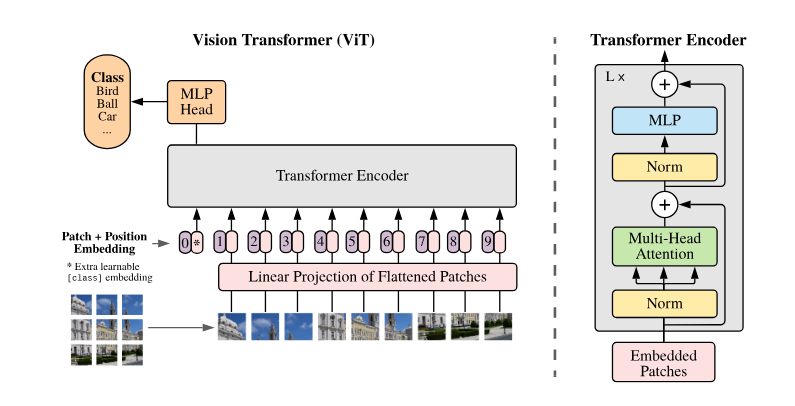
\includegraphics[width=1\textwidth]{images/vit-architecture.png}
    \caption{The Vision Transformer (ViT) architecture from \cite{alexey2020image}. On the left the model architecture while on the right the Transformer encoder block architecture from \cite{vaswani2017attention}.}
    \label{fig:vit-architecture}
\end{figure*}

\section{Architecture}

In recent years, the Transformer architecture originally developed for natural language processing has been successfully applied to computer vision tasks. The Vision Transformer (ViT) rethinks image classification by treating an image as a sequence of patches, much like tokens in a sentence, and processes them using standard Transformer blocks. In this chapter, we detail the architecture of the Vision Transformer and provide the mathematical foundations underlying its design.

\subsection{Overview}
The Vision Transformer (ViT) adapts the Transformer architecture originally developed for natural language processing to image classification tasks. Instead of processing an image as a whole, ViT divides it into a sequence of patches (analogous to tokens) and processes these patches through a stack of Transformer encoder blocks. The key steps in the ViT pipeline are:

\begin{enumerate}
    \item \textbf{Image Patch Embedding}: The input image is divided into fixed-size patches that are flattened and projected into a latent space.
    \item \textbf{Positional Encoding}: Since Transformers are permutation-invariant, positional embeddings are added to the patch embeddings.
    \item \textbf{Transformer Encoder}: A series of Transformer encoder blocks processes the sequence of embeddings using self-attention and feed-forward networks.
    \item \textbf{Classification Head}: The encoder output is used by a classification head for the final prediction.
\end{enumerate}

\subsection{Image Patch Embedding}

\textbf{Patch Extraction}

Given an input image 
\begin{equation}
    \mathbf{X} \in \mathbb{R}^{H \times W \times C},
\end{equation}
where \(H\) and \(W\) denote the height and width of the image, and \(C\) denotes the number of channels, the image is divided into \(N\) patches of size \(P \times P\). Hence, the number of patches is:
\begin{equation}
N = \frac{HW}{P^2}.
\end{equation}

\textbf{Flattening and Linear Projection}

Each patch, denoted as \(\mathbf{x}_p \in \mathbb{R}^{P \times P \times C}\), is flattened into a vector of dimension \(P^2 \cdot C\). A learnable linear projection (implemented as a fully connected layer) maps this vector into a \(D\)-dimensional embedding space:

\begin{equation}
    \mathbf{z}_p = \mathbf{W}_e \mathbf{x}_p + \mathbf{b}_e
\end{equation}

where $\mathbf{W}_e \in \mathbb{R}^{D \times (P^2 \cdot C)} \text{ and } \mathbf{b}_e \in \mathbb{R}^{D}$.

After processing all patches, we obtain a sequence of embeddings:

\begin{equation}
\mathbf{Z} = \left[\mathbf{z}_1, \mathbf{z}_2, \dots, \mathbf{z}_N\right] \in \mathbb{R}^{N \times D}.
\end{equation}

%%%%%%%%%%%%%%%%%%%%%%%%%%%%%%%%%%%%%%%%%%%%%%%%%%
\subsection{Positional Encoding}

Transformers do not inherently capture the order or spatial structure of input data. To inject spatial information, learnable positional embeddings are added to the patch embeddings. Let:
\begin{equation}
\mathbf{E}_{\text{pos}} \in \mathbb{R}^{N \times D}
\end{equation}

be a set of positional embeddings. The combined input to the Transformer encoder is then:
\begin{equation}
\mathbf{Z}_0 = \mathbf{Z} + \mathbf{E}_{\text{pos}}.
\end{equation}

In some implementations, a special class token \(\mathbf{z}_{\text{cls}} \in \mathbb{R}^{D}\) is prepended to the sequence:
\begin{equation}
\mathbf{Z}_0 = \left[\mathbf{z}_{\text{cls}}, \mathbf{z}_1, \dots, \mathbf{z}_N \right].
\end{equation}

%%%%%%%%%%%%%%%%%%%%%%%%%%%%%%%%%%%%%%%%%%%%%%%%%%
\subsection{Transformer Encoder Blocks}

The Vision Transformer uses a stack of \(L\) Transformer encoder blocks. Each block is composed of two main components: the Multi-Head Self-Attention (MHSA) mechanism and a Feed-Forward Network (FFN). Layer normalization (LN) and residual connections are applied around each component.

\textbf{Multi-Head Self-Attention (MHSA)}

Let \(\mathbf{Z}^{(l-1)} \in \mathbb{R}^{M \times D}\) be the input to the \(l\)-th encoder block, where \(M\) is the number of tokens (including the class token if used).

\textbf{Query, Key, and Value}

The input is projected into query (\(\mathbf{Q}\)), key (\(\mathbf{K}\)), and value (\(\mathbf{V}\)) matrices using learnable projection matrices \(\mathbf{W}_Q, \mathbf{W}_K, \mathbf{W}_V \in \mathbb{R}^{D \times D}\):

\begin{equation}
\mathbf{Q} = \mathbf{Z}^{(l-1)} \mathbf{W}_Q, \quad \mathbf{K} = \mathbf{Z}^{(l-1)} \mathbf{W}_K, \quad \mathbf{V} = \mathbf{Z}^{(l-1)} \mathbf{W}_V.
\end{equation}

For multi-head attention, these are divided into \(h\) heads. For head \(i\) (\(i=1,\dots,h\)), we have:
\begin{equation}
    \mathbf{Q}_i, \mathbf{K}_i, \mathbf{V}_i \in \mathbb{R}^{M \times d}, \quad \text{with } d = \frac{D}{h}.
\end{equation}

\textbf{Scaled Dot-Product Attention}

For head \(i\), the attention is computed as:
\[
\text{Attention}_i(\mathbf{Q}_i, \mathbf{K}_i, \mathbf{V}_i) = \text{softmax}\left(\frac{\mathbf{Q}_i \mathbf{K}_i^\top}{\sqrt{d}}\right) \mathbf{V}_i.
\]
The scaling by \(\sqrt{d}\) ensures numerical stability.

\textbf{Concatenation and Final Projection}

The outputs from all \(h\) heads are concatenated and projected:
\[
\text{MultiHead}(\mathbf{Q}, \mathbf{K}, \mathbf{V}) = \text{Concat}\left(\text{Attention}_1, \dots, \text{Attention}_h\right) \mathbf{W}_O,
\]
with \(\mathbf{W}_O \in \mathbb{R}^{D \times D}\) being a learned projection matrix.

\textbf{Residual Connection and Normalization}

A residual connection and layer normalization are applied:
\[
\mathbf{Z}^{\prime(l)} = \text{LN}\left(\mathbf{Z}^{(l-1)} + \text{MultiHead}(\mathbf{Q}, \mathbf{K}, \mathbf{V})\right).
\]

\textbf{Feed-Forward Network (FFN)}

Each encoder block contains a two-layer FFN applied to each token independently:

\begin{equation}
    \text{FFN}(\mathbf{z}) = \text{GELU}\left(\mathbf{z} \mathbf{W}_1 + \mathbf{b}_1\right) \mathbf{W}_2 + \mathbf{b}_2,
\end{equation}

where:
\begin{itemize}
    \item \(\mathbf{W}_1 \in \mathbb{R}^{D \times D_{\text{ff}}}\),
    \item \(\mathbf{W}_2 \in \mathbb{R}^{D_{\text{ff}} \times D}\),
    \item \(D_{\text{ff}}\) is the dimension of the hidden layer,
    \item GELU is the Gaussian Error Linear Unit activation.
\end{itemize}

A residual connection and layer normalization follow:
\begin{equation}
    \mathbf{Z}^{(l)} = \text{LN}\left(\mathbf{Z}^{\prime(l)} + \text{FFN}(\mathbf{Z}^{\prime(l)})\right).
\end{equation}

%%%%%%%%%%%%%%%%%%%%%%%%%%%%%%%%%%%%%%%%%%%%%%%%%%
\subsection{Classification Head}

For classification tasks, the output corresponding to the class token (or a pooled representation of all tokens) is used. For instance, if a class token \(\mathbf{z}_{\text{cls}}\) is used, the final prediction is obtained as:

\begin{equation}
\hat{y} = \text{softmax}\left(\mathbf{W}_c \mathbf{z}_{\text{cls}} + \mathbf{b}_c\right),
\end{equation}

where \(\mathbf{W}_c \in \mathbb{R}^{K \times D}\) and \(\mathbf{b}_c \in \mathbb{R}^{K}\) are the weights and bias of the classification layer, and \(K\) is the number of classes. Alternatively, a global average pooling can be applied to the token embeddings before the linear projection.

%%%%%%%%%%%%%%%%%%%%%%%%%%%%%%%%%%%%%%%%%%%%%%%%%%


\section{Tiny Vision Transformer (Tiny ViT)}

\begin{table}[htbp]
  \small
  \centering
  \caption{Parameters of the TinyViT Model for CIFAR-10}
  \begin{tabular}{@{}ll@{}}
    \toprule
    \textbf{Parameter} & \textbf{Value} \\
    \midrule
    Number of Classes & 10 \\
    Embedding Dimension & 128 \\
    Image Size & 32 \\
    Patch Size & 4 \\
    Input Channels & 3 \\
    Number of Attention Heads & 8 \\
    Number of Transformer Layers & 6 \\
    MLP Hidden Dimension & 512 \\
    \bottomrule
  \end{tabular}
\end{table}

The Vision Transformer (ViT) has proven to be highly effective for image classification by using self attention mechanisms instead of conventional convolutional operations. Since the original Vision Transformer requires large datasets and significant computational power, TinyViT is designed specifically for smaller datasets and demands less computation. To address this, a compact variant, Tiny Vision Transformer (TinyViT), has been implemented with modifications aimed at efficiency. TinyViT is designed to operate efficiently on smaller images such as 32x32 but can also be adapted for other resolutions like 96x96, dividing them into 4x4 patches, resulting in 64 tokens per image. These patches are projected into an embedding space of 128 dimensions, which serve as input to the Transformer encoder. The model consists of six Transformer layers with eight attention heads each, along with feed-forward networks featuring a hidden dimension of 512. These design choices allow for a balance between model capacity and computational feasibility, leading to approximately 1.21 million trainable parameters.

Compared to standard ViT models, which process high resolution images with larger patch sizes and higher embedding dimensions, TinyViT scales down key components while maintaining self attention’s effectiveness. Traditional ViT architectures often use embedding dimensions over 768 and deeper networks. By reducing the embedding dimension, the number of Transformer layers, and the patch size, TinyViT significantly lowers computational requirements while retaining essential representation learning capabilities.

The motivation behind TinyViT is to use the advantages of ViT while ensuring possibility for lower resolution datasets. Given CIFAR-10’s 32x32 images, a full-scale ViT model would be excessive. By optimizing model depth, embedding dimensions, and MLP hidden size, TinyViT ensures efficient training without compromising performance. The reduced number of parameters makes it compatible with standard GPUs and avoids excessive memory consumption.

\raggedbottom
\section{Datasets}
The experiments in this work utilize three widely recognized image classification benchmarks: CIFAR-10, CIFAR-100, and STL-10. The CIFAR-10 dataset contains 60,000 RGB 32x32 images divided into 10 classes, with 6,000 images per class, offering a balanced benchmark for evaluating basic recognition capabilities. CIFAR-100 shares the same total number of images as CIFAR-10 but includes 100 fine grained classes, each represented by 600 images, thereby introducing greater categorization complexity. STL-10 consists of 130,000 higher resolution 96x96 RGB images across 10 classes. These datasets collectively provide a multi-scale evaluation framework, testing the TinyViT architecture across varying class granularities, data volumes, and image resolutions.

\begin{figure}
    \centering
    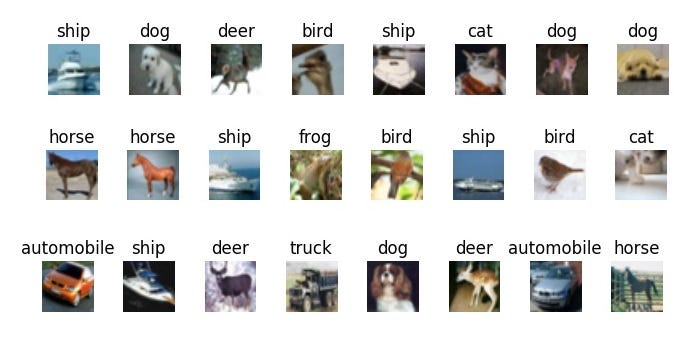
\includegraphics[width=0.5\textwidth]{images/cifar-10.jpg}
    \caption{CIFAR-10 dataset samples images and classes \cite{krizhevsky2009learning}.}
    \label{fig:datasets}
\end{figure}

The experiments uses standard train-test splits for all datasets: CIFAR-10 and CIFAR-100 each include 50,000 training and 10,000 test images, while STL-10 uses 5,000 labeled training images and 8,000 test samples. For CIFAR-10 and CIFAR-100, training data undergoes augmentation via random cropping (32x32 with 4 pixel padding) and horizontal flipping, followed by normalization using channel wise means (0.4914, 0.4822, 0.4465) and standard deviations (0.2470, 0.2435, 0.2616). Test images are directly normalized without augmentation. STL-10, with its higher 96x96 resolution, employs more extensive training augmentations: 12 padded random cropping, horizontal flipping, 15 degree rotations, color jittering (brightness, contrast, saturation), and random grayscaling (10\% probability), normalized with dataset specific statistics (means: 0.4467, 0.4398, 0.4066; stds: 0.2603, 0.2566, 0.2713). Test sets for all datasets apply only resizing, tensor conversion, and identical normalization to ensure evaluation consistency. These transformations balance generalization during training and standardization during testing.
\section{Evaluation Metrics}

\section{Conclusion and Future Work}
In this chapter a conclusion is drawn from the results obtained in the previous chapter. The chapter also discusses the future work that can be done to improve the model.

\subsection{Conclusion}
In conclusion, the implementation of the Tiny ViT architecture has shown promising results, often performing on par with, and occasionally surpassing, standard Convolutional Neural Networks (CNNs) in image recognition tasks. This achievement underscores the potential of Vision Transformers (ViTs) as a robust alternative to the well established CNNs, offering exploration beyond conventional CNN implementations. While we did not achieve the performance levels of the standard ViT architecture, primarily due to the absence of large scale datasets for pre training and subsequent transfer learning, we successfully demonstrated that a scaled down ViT architecture can obtain good results without the need for massive datasets.
\subsection{Future Work}
Future work to evaluate the performance of the proposed tiny Vision Transformer (ViT) architecture on two key computer vision tasks: object detection and semantic segmentation. Specifically, the tiny ViT could be implemented for frameworks like DETR \cite{carion2020end} for object detection and Segmenter \cite{strudel2021segmenter} for segmentation, enabling a direct comparison with simpler CNN based architectures traditionally used for these tasks. Additionally, the Tiny ViT architecture could be further optimized by exploring different hyperparameters, such as the number of layers, hidden units, and attention heads, to improve its performance.

\bibliographystyle{apalike}
\bibliography{bibliography.bib}

\end{document}
